\chapter{Preliminaries}{}{}
\label{CH:PRELIM}%

This chapter provides a brief background of the video 
super-resolution (VSR), diffusion models for image restoration, 
and wavelet transforms for visual tasks. 

%Section 2.1 introduces an overview of VSR and details of 
%essential modules related to our work; temporal alignment and 
%feature aggregation. Section 2.2 gives the theoretical 
%background of diffusion models and some of their applications 
%in image restoration. Section 2.3 introduces wavelet transforms 
%and their use in deep learning frameworks.

%===================== Overview of VSR ===================%
\section{Overview of Video Super-Resolution}

Video super-resolution (VSR) systems have been deeply explored 
in the computer vision field and have been applied in various 
applications. According to Liu and Sun \cite{liu2013vid4}, the 
VSR problem is fundamentally an inverse problem of recovering 
high-resolution (HR) frames from their low-resolution (LR) 
counterparts. They formulated the problem under a Bayesian 
framework with priors over both spatial and temporal 
dimensions. Subsequently, deep learning-based formulations were 
established \cite{kappeler2016vsrnet} and the focus shifted 
toward learning effective spatial-temporal representations 
from data. However, satisfactory restoration of fine textural 
details remained dominant \cite{caballero2017vespcn} as a 
challenge in VSR. Many studies also have been conducted on 
perceptual super-resolution with the idea that pixel-level 
fidelity cannot fully capture human visual perception 
\cite{ledig2017srgan, wang2018esrgan, wang2021realbasicvsr, 
chan2022basicvsrplusplus, rota2024stablevsr}.


The three main modules in the VSR system are as follows: 
temporal alignment, feature aggregation, and reconstruction. 
Alignment methods such as optical flow estimation 
\cite{teed2020raft}, deformable convolution 
\cite{dai2017deformable}, and recurrent propagation 
\cite{chan2021basicvsr} have been applied to align features 
across adjacent frames. After that, multi-frame features are 
aggregated by a feature aggregator and these features are 
upsampled into HR resolution by a reconstruction module. 
Traditionally, hand-crafted upsampling on the image and 
self-similarity of patches played a significant role in VSR. 
Previous work, sparse coding \cite{yang2010sparsecoding}, 
dictionary learning \cite{zeyde2010dictionary}, Bayesian 
inference \cite{liu2013vid4}, and self-exemplar methods 
\cite{glasner2009self} were mainly researched. These methods 
have been usually experimented with under controlled datasets 
such as Vid4 \cite{liu2013vid4}, SPMCS \cite{tao2017spmcs}, 
UDM10 \cite{yi2019udm10}, and other constrained datasets. 
Extracted features from those algorithms were upsampled by 
linear regression, polynomial fitting, and other shallow 
classification models. Especially, the combination of optical 
flow alignment which provides pixel-level correspondence across 
frames, and sparse coding which exploits the redundancy in 
natural image patches has been widely researched.


Large-scale video datasets such as REDS \cite{nah2019reds}, 
Vimeo-90K \cite{xue2019vimeo}, and YouTube-8M 
\cite{abu2016youtube8m} were gathered as the deep learning 
challenges for VSR started. However, training on large-scale 
unconstrained dataset requires substantial memory and 
computation. To address this problem, convolutional neural 
network (CNN)-based models have been employed for VSR tasks. 
It is because CNN \cite{lecun1998} can extract deeper and more 
spatial inductive biases information. Moreover, other 
approaches like recurrent network, sliding-window architecture, 
and transformer-based models are also widely researched in 
VSR tasks.


As shown in Figure~\ref{fig:vsr_pipeline}, the recent VSR 
process has three stages: Pre-processing, Feature learning, 
and Reconstruction. In the pre-processing stage, temporal 
alignment, motion compensation, and frame normalization are 
proposed. Some models use sliding-window without explicit 
alignment depending on their design choice. In the feature 
learning stage, various deep learning-based models like CNN, 
RNN, and Transformer have been applied to extract effective 
features without losing spatial-temporal prior information. 
In reconstruction, the network upsamples extracted features 
into one of the HR resolutions. In recent work, however, 
feature extraction and feature reconstruction have been 
separated. This VSR pipeline can do end-to-end learning from 
LR input to HR output. Due to this process, regularizing 
learning is possible by the loss function.


\begin{figure}[htbp] 
\centering
%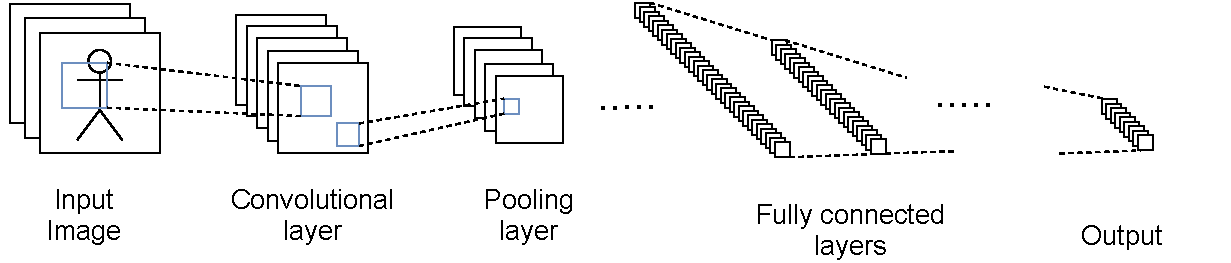
\includegraphics[width=\textwidth]{fig/general_cnn.pdf}
\caption{The general pipeline of Video Super-Resolution task.}
\label{fig:vsr_pipeline}
\end{figure}


Many VSR tasks have presented promising results. However, 
still, there are limitations. VSR with deep learning networks 
often falls into the perception-distortion trade-off problem. 
Although LR frames are reconstructed well in pixel-level 
fidelity (PSNR/SSIM), their perceptual quality drops on test 
sequences. One way to solve this issue is by applying a 
generative model trained on large-scale image datasets. 
Outputs from CNN-based regression models are over-smoothed 
images that lack categories: textural details, sharp edges, 
high-frequency patterns, and other fine structures. On the 
other hand, outputs from generative models such as those 
based on diffusion are sharper images. Examples of generative 
VSR are RealBasicVSR \cite{wang2021realbasicvsr} and StableVSR 
\cite{rota2024stablevsr}. However, generative VSR (diffusion 
models) have higher temporal flickering than CNN-based VSR 
models. As applying generative models may introduce 
inter-frame inconsistency, frequency-aware conditioning is 
needed. Therefore, frequency-domain priors can play a key 
role in this situation.


%-------------- Subsection ---------------%
\subsection{VSR issues related to methods and datasets}

Extracting high-frequency details from low-resolution video 
frames and maintaining temporal consistency is challenging. 
Table~\ref{tab:vsr_issues_methods} illustrates various 
approaches that have been proposed to address this problem. 
Researchers usually studied alignment mechanisms to maximize 
the temporal information utilization \cite{chan2021basicvsr, 
chan2022basicvsrplusplus, wang2019edvr}. Also, augmentation 
strategy and ensemble learning has been proposed 
\cite{wang2021realbasicvsr, jo2018dup, isobe2020rsdn, 
liang2024vrt}.


\begin{sidewaystable}[htbp]
\caption{Various issues existing in VSR methods}
\centering
\resizebox{\textwidth}{!}{
    \begin{tabular}{|l|l|l|}
    \hline
    \textbf{Method} & \textbf{Issues} & \textbf{Reference} \\ 
    \hline \hline
    Augmentation strategy & overfitting on synthetic degradation 
    & \cite{wang2021realbasicvsr} \\ \hline
    Ensemble learning & high computational cost and redundancy 
    & \cite{jo2018dup} \\ \hline
    & difficulty in capturing long-range temporal dependencies 
    & \cite{chan2022basicvsrplusplus}, \cite{liang2024vrt}, 
    \cite{wang2019edvr} \\ \cline{2-3}
    Alignment mechanism & degradation due to inaccurate optical flow 
    & \cite{chan2021basicvsr} \\ \cline{2-3}
    & VSR-specific alignment is required & \cite{wang2019edvr} \\ 
    \cline{2-3}
    & difficulty in learning from large motion frames 
    & \cite{isobe2020rsdn} \\ \cline{1-3}
    Loss function & over-smoothing in pixel-level losses 
    & \cite{ledig2017srgan} \\ \cline{2-3}
    & temporal consistency requires explicit supervision 
    & \cite{chu2020temporal} \\ \cline{1-3}
    Other approaches & perception-distortion trade-off problem 
    & \cite{blau2018perception}, \cite{wang2021realbasicvsr}, 
    \cite{rota2024stablevsr} \\ \hline
    \end{tabular}}
\label{tab:vsr_issues_methods}
\end{sidewaystable}


On the other hand, training VSR datasets are challenging. Many 
types of research have been studied focusing on VSR datasets. 
Video datasets have issues including unrealistic synthetic 
degradation, limited motion diversity, content imbalance, etc. 
Especially, real-world video datasets have differences in 
compression artifacts, sensor noise, and motion blur. As shown 
in Table~\ref{tab:vsr_issues_data}, we discuss the recent 
studies dealing with the video data problem and enhancing 
performance in VSR tasks.


\begin{sidewaystable}[htbp]
\caption{Various issues related to datasets}
\centering
\resizebox{\textwidth}{!}{
\begin{tabular}{|c|c|c|c|}
\hline
& \textbf{\begin{tabular}[c]{@{}c@{}}dataset\\ (size, resolution, content)\end{tabular}} 
& \textbf{issues} & \textbf{ref} \\ 
\hline \hline
& & limited motion diversity & \cite{nah2019reds} \\ \cline{3-4}
& \begin{tabular}[c]{@{}c@{}}REDS\\ (270 seqs, 720p, dynamic)\end{tabular} 
& synthetic bicubic degradation gap from real-world content 
& \cite{wang2021realbasicvsr} \\ \cline{2-4}
synthetic & \begin{tabular}[c]{@{}c@{}}Vimeo-90K\\ (90K seqs, 256$\times$448, mixed)\end{tabular} 
& low-resolution ground truth limits perceptual evaluation 
& \cite{xue2019vimeo} \\ \cline{3-4}
& & content bias toward natural scenes & \cite{liang2024vrt} \\ 
\cline{2-4}
& \begin{tabular}[c]{@{}c@{}}Vid4 / SPMCS / UDM10\\ (small-scale, mixed)\end{tabular} 
& small-scale evaluation with limited generalization 
& \cite{liu2013vid4}, \cite{tao2017spmcs}, \cite{yi2019udm10} \\ 
\hline
\multicolumn{1}{|l|}{real-world} 
& \begin{tabular}[c]{@{}c@{}}VideoLQ\\ (50 clips, real-world)\end{tabular} 
& no ground truth for quantitative evaluation 
& \cite{wang2021realbasicvsr} \\ \cline{3-4}
\multicolumn{1}{|l|}{} & & complex degradation modeling required 
& \cite{wang2021realbasicvsr} \\ \hline
\end{tabular}}
\label{tab:vsr_issues_data}
\end{sidewaystable}

%===================== Overview of Diffusion ===================%
\section{Overview of Diffusion Models for Image Restoration}

As the solutions to image restoration problems aligned with 
generative scenarios, Ho \emph{et al.} and Saharia \emph{et al.} 
proposed that probabilistic generative modeling is required 
in future image restoration tasks 
\cite{ho2020ddpm, saharia2022sr3}. Therefore, the diffusion 
model technique can be reasonably applied for super-resolution 
tasks.

A diffusion model defines a forward process that progressively 
adds Gaussian noise to a clean image $x_0$ over $T$ timesteps:
\begin{equation}
    q(x_t \mid x_{t-1}) = 
    \mathcal{N}\big(x_t; \sqrt{1-\beta_t}\, x_{t-1},\, 
    \beta_t \mathbf{I}\big),
    \label{eq:forward_process}
\end{equation}
where $\{\beta_t\}_{t=1}^T$ is a predefined variance schedule. 
By the reparameterization trick, the marginal distribution at 
any timestep $t$ admits a closed-form expression:
\begin{equation}
    q(x_t \mid x_0) = 
    \mathcal{N}\big(x_t; \sqrt{\bar{\alpha}_t}\, x_0,\, 
    (1-\bar{\alpha}_t)\mathbf{I}\big),
    \label{eq:closed_forward}
\end{equation}
where $\alpha_t = 1 - \beta_t$ and 
$\bar{\alpha}_t = \prod_{s=1}^{t} \alpha_s$. The reverse 
process is parameterized by a neural network 
$\epsilon_\theta(x_t, t)$ that predicts the noise component at 
each timestep, trained via the simplified objective:
\begin{equation}
    \mathcal{L}_{\mathrm{simple}} = 
    \mathbb{E}_{t, x_0, \epsilon} \!\left[ 
    \big\| \epsilon - \epsilon_\theta(x_t, t) \big\|^2 \right],
    \label{eq:ddpm_loss}
\end{equation}
where $\epsilon \sim \mathcal{N}(\mathbf{0}, \mathbf{I})$ is 
the noise sampled during the forward process. After training, 
high-quality samples are generated by iteratively denoising 
from $x_T \sim \mathcal{N}(\mathbf{0}, \mathbf{I})$ following 
the learned reverse trajectory.

In this section, we discuss an overview of image restoration 
systems using diffusion models with respect to single-image 
super-resolution and video super-resolution. Research that 
targets single-image diffusion usually focuses on conditioning 
the denoising process on the low-resolution input or on 
extracted spatial features. On the other hand, research that 
targets video super-resolution focuses on extending the 
diffusion process with temporal context across adjacent frames.


%-------------- Subsection ---------------%
\subsection{Single-image diffusion-based super-resolution}

Image restoration tasks using diffusion models generally focused 
on two techniques: pixel-space diffusion and latent-space 
diffusion. Early diffusion-based super-resolution tasks had 
suffered from the high computational cost of pixel-space 
denoising on high-resolution images until the appearance of 
latent diffusion frameworks. Therefore, utilizing as efficient 
denoising as possible during inference and achieving reasonable 
perceptual quality were the main issues \cite{ho2020ddpm}.

Rombach \emph{et al.} proposed Latent Diffusion Models (LDM) 
that perform the diffusion process in a compressed latent space 
to reduce computational cost \cite{rombach2022ldm}. Given a 
pre-trained VAE encoder $\mathcal{E}$ and decoder $\mathcal{D}$, 
the input image $x$ is first compressed into a latent 
representation $z = \mathcal{E}(x)$, and the diffusion process 
operates on $z$ instead of the pixel space:
\begin{equation}
    \mathcal{L}_{\mathrm{LDM}} = 
    \mathbb{E}_{t, z_0, \epsilon, c} \!\left[ 
    \big\| \epsilon - \epsilon_\theta(z_t, t, c) \big\|^2 \right],
    \label{eq:ldm_loss}
\end{equation}
where $c$ is the conditioning input (e.g., text, class label, 
or low-resolution image). The denoised latent $\hat{z}_0$ is 
then decoded back to the pixel space via $\hat{x} = 
\mathcal{D}(\hat{z}_0)$. This compression reduces the spatial 
dimension by $\sim$8$\times$ in each axis, drastically lowering 
computational cost.

Saharia \emph{et al.} suggested research that focused on the 
conditional generation problem to deploy diffusion models in 
real-world restoration tasks \cite{saharia2022sr3}. They 
proposed SR3 (Super-Resolution via Repeated Refinement), thus 
tackling the problem of conditional generation on low-resolution 
inputs. Wang \emph{et al.} insisted that diffusion priors and 
controllability cause performance variation in image restoration 
\cite{wang2024exploiting}. Wang \emph{et al.} considered the 
pre-trained Stable Diffusion as the prior, and the controllable 
generation as the testing scenario \cite{wang2024exploiting}. 
To address the problem of controllability, they proposed 
StableSR that included a time-aware encoder with feature-level 
conditioning. Moreover, Zhang \emph{et al.} proposed ControlNet, 
which extends pre-trained diffusion models with an additional 
conditioning branch \cite{zhang2023controlnet}. The ControlNet 
output is integrated into the U-Net via zero-initialized 
convolutions:
\begin{equation}
    y = \mathcal{F}(x; \theta) + 
    \mathcal{Z}\big(\mathcal{F}(x + \mathcal{Z}(c; \theta_{z1}); 
    \theta_c); \theta_{z2}\big),
    \label{eq:controlnet}
\end{equation}
where $\mathcal{F}(\cdot; \theta)$ is the frozen pre-trained 
U-Net block, $\mathcal{Z}(\cdot; \theta_z)$ is a 
zero-initialized convolution layer, and $c$ is the conditioning 
signal. With this architecture, the perceptual quality is 
improved and the artifact generation is suppressed.


%-------------- Subsection ---------------%
\subsection{Video super-resolution with diffusion models}

Liu \emph{et al.} explored the generalization ability of 
diffusion algorithms on recovering high-resolution video frames 
with limited temporal context \cite{liu2024videosr}. Starting 
from this review study, many approaches for incorporating 
temporal coherence into diffusion-based video super-resolution 
have been studied, especially adjacent-frame conditioning. Yang 
\emph{et al.} proposed motion-guided latent diffusion network 
(MGLD-VSR) for real-world video super-resolution with joint 
learning \cite{yang2023motion}. Through joint learning, it 
prevents the model from overfitting to specific motion patterns. 
Zhou \emph{et al.} proposed text-guided diffusion for video 
super-resolution \cite{zhou2024upscale}. They used text prompts 
on both training and testing. Two methods (text conditioning 
and temporal attention) are adopted to enable the model to 
acquire knowledge from large-scale text-image pairs available 
in other scenarios (source domain), and then transfer the 
knowledge to the scenario where it works (target domain), 
reconstructing high-resolution videos with only a few text 
prompts.

However, Rota \emph{et al.} proposed a novel video 
super-resolution framework called StableVSR, which was trained 
to obtain transferable temporal warping prior with cascaded 
ControlNet modules with a shared parameter 
\cite{rota2024stablevsr}. Specifically, the conditioning input 
$c$ in Equation~\ref{eq:controlnet} is constructed from the 
adjacent frames $\{I^{LR}_{t-1}, I^{LR}_{t+1}\}$ warped to the 
current timestep via RAFT-based optical flow 
\cite{teed2020raft}:
\begin{equation}
    c_t = \big[ \mathcal{W}(I^{LR}_{t-1} \to t) \,\big\|\, 
    \mathcal{W}(I^{LR}_{t+1} \to t) \big],
    \label{eq:stablevsr_cond}
\end{equation}
where $\mathcal{W}(\cdot \to t)$ denotes optical flow-based 
warping toward the current timestep $t$, and $\|$ is 
channel-wise concatenation. With this approach, Rota \emph{et 
al.} pointed out the burden of integrating temporal context 
into pre-trained diffusion models and solved the limitations 
of single-image diffusion approaches and motion-guided 
diffusion methods. The transferable temporal features were 
easily adapted to novel video super-resolution tasks. In 
particular, a bidirectional sampling strategy was designed to 
take full advantage of forward and backward temporal directions 
during denoising. In this way, StableVSR could alleviate 
inter-frame inconsistency due to limited temporal context. 
StableVSR was trained with adjacent-frame warping for video 
super-resolution tasks.